\documentclass[12pt]{book}

\usepackage{natbib} % Tidies up citation numbers.
\usepackage[utf8]{inputenc}
\usepackage{graphicx}
\usepackage{pythonhighlight}
\usepackage{listingsutf8}
\usepackage{float}

%\def\UrlBreaks{\do\/\do-}
\usepackage[T1]{fontenc}
\usepackage{url}
\usepackage{breakurl}

\usepackage{pdfpages}

\lstset{
  extendedchars=true,
  language=java,
  basicstyle=\tiny\ttfamily,
  showspaces=false,
  showstringspaces=false,
    literate=
     {É}{{\'E}}{1}%
      {Á}{{\'A}}{1}%
      {Ã}{{\~A}}{1}%
      {Â}{{\^A}}{1}%
      {À}{{\`A}}{1}%
      {Ç}{{\,C}}{1}%
      {Ó}{{\'O}}{1}%
      {Í}{{\'I}}{1}%
      {Õ}{{\~O}}{1}%
      {Ú}{{\'U}}{1}%
      {ú}{{\'u}}{1}%
      {é}{{\'e}}{1}%
      {á}{{\'a}}{1}%
      {ã}{{\~a}}{1}%
      {à}{{\`a}}{1}%
      {â}{{\^a}}{1}%
      {ç}{{\,c}}{1}%
      {ó}{{\'o}}{1}%
      {í}{{\'i}}{1}%
      {õ}{{\~o}}{1}%
}

\definecolor{gray}{rgb}{0.4,0.4,0.4}
\definecolor{darkblue}{rgb}{0.0,0.0,0.6}
\definecolor{cyan}{rgb}{0.0,0.6,0.6}

\lstdefinelanguage{XML}
{
 numbers=left,
 numberstyle=\tiny,
 stepnumber=1,
 numbersep=8pt,
 morestring=[b]",
 morestring=[s]{>}{<},
 morecomment=[s]{<?}{?>},
 stringstyle=\color{black},
 identifierstyle=\color{darkblue},
 keywordstyle=\color{cyan},
 morekeywords={xmlns,version,type}% list your attributes here
}

\colorlet{punct}{red!60!black}
\definecolor{background}{HTML}{EEEEEE}
\definecolor{delim}{RGB}{20,105,176}
\colorlet{numb}{magenta!60!black}

\lstdefinelanguage{json}{
    basicstyle=\tiny\ttfamily,
    numbers=left,
    numberstyle=\tiny,
    stepnumber=1,
    numbersep=8pt,
    showstringspaces=false,
    breaklines=true,
    frame=lines,
    backgroundcolor=\color{background},
    literate=
     *{É}{{\'E}}{1}%
      {Á}{{\'A}}{1}%
      {Ã}{{\~A}}{1}%
      {Â}{{\^A}}{1}%
      {À}{{\`A}}{1}%
      {Ç}{{\,C}}{1}%
      {Ó}{{\'O}}{1}%
      {Í}{{\'I}}{1}%
      {Õ}{{\~O}}{1}%
      {Ú}{{\'U}}{1}%
      {ú}{{\'u}}{1}%
      {é}{{\'e}}{1}%
      {á}{{\'a}}{1}%
      {ã}{{\~a}}{1}%
      {à}{{\`a}}{1}%
      {â}{{\^a}}{1}%
      {ç}{{\,c}}{1}%
      {ó}{{\'o}}{1}%
      {í}{{\'i}}{1}%
      {õ}{{\~o}}{1}%
     {0}{{{\color{numb}0}}}{1}
      {1}{{{\color{numb}1}}}{1}
      {2}{{{\color{numb}2}}}{1}
      {3}{{{\color{numb}3}}}{1}
      {4}{{{\color{numb}4}}}{1}
      {5}{{{\color{numb}5}}}{1}
      {6}{{{\color{numb}6}}}{1}
      {7}{{{\color{numb}7}}}{1}
      {8}{{{\color{numb}8}}}{1}
      {9}{{{\color{numb}9}}}{1}
      {:}{{{\color{punct}{:}}}}{1}
      {,}{{{\color{punct}{,}}}}{1}
      {\{}{{{\color{delim}{\{}}}}{1}
      {\}}{{{\color{delim}{\}}}}}{1}
      {[}{{{\color{delim}{[}}}}{1}
      {]}{{{\color{delim}{]}}}}{1},
}

\lstdefinelanguage{SPARQL}{
    basicstyle=\tiny\ttfamily,
    numbers=left,
    numberstyle=\tiny,
    stepnumber=1,
    numbersep=8pt,
    showstringspaces=false,
    breaklines=true,
    frame=lines,
    backgroundcolor=\color{background},
    literate=
     {É}{{\'E}}{1}%
      {Á}{{\'A}}{1}%
      {Ã}{{\~A}}{1}%
      {Â}{{\^A}}{1}%
      {À}{{\`A}}{1}%
      {Ç}{{\,C}}{1}%
      {Ó}{{\'O}}{1}%
      {Í}{{\'I}}{1}%
      {Õ}{{\~O}}{1}%
      {Ú}{{\'U}}{1}%
      {ú}{{\'u}}{1}%
      {é}{{\'e}}{1}%
      {á}{{\'a}}{1}%
      {ã}{{\~a}}{1}%
      {à}{{\`a}}{1}%
      {â}{{\^a}}{1}%
      {ç}{{\,c}}{1}%
      {ó}{{\'o}}{1}%
      {í}{{\'i}}{1}%
      {õ}{{\~o}}{1},%
  morekeywords={
    SELECT,CONSTRUCT,DESCRIBE,ASK,WHERE,FROM,NAMED,PREFIX,BASE,OPTIONAL,
    FILTER,GRAPH,LIMIT,OFFSET,SERVICE,UNION,EXISTS,NOT,BINDINGS,MINUS,a
  }
}

\lstdefinelanguage{overpassQL}{
    basicstyle=\tiny\ttfamily,
    numbers=left,
    numberstyle=\tiny,
    stepnumber=1,
    numbersep=8pt,
    showstringspaces=false,
    breaklines=true,
    frame=lines,
    backgroundcolor=\color{background}
}

\lstset{language=R,
    literate=
    {<-}{{$\gets$}}1%
     {É}{{\'E}}{1}%
      {Á}{{\'A}}{1}%
      {Ã}{{\~A}}{1}%
      {Â}{{\^A}}{1}%
      {À}{{\`A}}{1}%
      {Ç}{{\,C}}{1}%
      {Ó}{{\'O}}{1}%
      {Í}{{\'I}}{1}%
      {Õ}{{\~O}}{1}%
      {Ú}{{\'U}}{1}%
      {ú}{{\'u}}{1}%
      {é}{{\'e}}{1}%
      {á}{{\'a}}{1}%
      {ã}{{\~a}}{1}%
      {à}{{\`a}}{1}%
      {â}{{\^a}}{1}%
      {ç}{{\,c}}{1}%
      {ó}{{\'o}}{1}%
      {í}{{\'i}}{1}%
      {õ}{{\~o}}{1},%
    basicstyle=\tiny\ttfamily,
    stringstyle=\color{red},
    otherkeywords={0,1,2,3,4,5,6,7,8,9},
    morekeywords={TRUE,FALSE},
    deletekeywords={data,frame,length,as,character},
    keywordstyle=\color{blue},
    commentstyle=\color{red},
}

\usepackage[brazil]{babel}  
\usepackage{xcolor}
%xcolor v2.12 (2016/05/11)384  Colors by Name4.1  Base colors (always available)black blue brown cyan darkgray gray green lightgray lime magenta olive orange pink purple red teal violet white yellow

\usepackage[nopostdot]{glossaries}
\setglossarystyle{altlist}
\PassOptionsToPackage{hyphens}{url}
\usepackage [colorlinks = true,
            linkcolor = blue,
            urlcolor  = blue,
            citecolor = blue,
            anchorcolor = blue]{hyperref} 

% gerador de lero-lero
\usepackage{lipsum}

\usepackage{pdfpages}

\newenvironment{itquote}
{\begin{quote}\itshape}
{\end{quote}}

\usepackage[commentmarkup=todo]{changes}

\usepackage{datetime2}

\usepackage{booktabs}

\usepackage{caption}
\input{packages-estudantes}

% define cores personalizadas para o texto de cada autor
\usepackage
%[final]
{changes}
%\usepackage{changes}
%\url{https://ctan.org/pkg/changes}

\definechangesauthor[name={Jorge Henrique Cabral Fernandes}, color=orange]{jhcf} % git-user: jhcf

\definechangesauthor[name={Alexsander Correa de Oliveira}, color=black]{KvotheKS} % git-user: KvotheKS OK

\definechangesauthor[name={Allann Gois Hoffmann}, color=orange]{AllannH} % git-user: AllannH OK

\definechangesauthor[name={André Larrosa Chimpliganond}, color=orange]{andrelarrosacrypt} % git-user: andrelarrosacrypt OK

\definechangesauthor[name={André Cássio Barros de Souza}, color=green]{andreloff} % git-user: andreloff OK

\definechangesauthor[name={Bruno Sanguinetti Regadas de Barros}, color=blue]{Jaxiii} % git-user: Jaxiii OK

\definechangesauthor[name={Enzo Nunes Leal Sampaio}, color=orange]{enzodevs2000} % git-user: enzodevs2000 OK

\definechangesauthor[name={Felipe Gomes Paradas}, color=pink]{fparadas} % git-user: fparadas OK

\definechangesauthor[name={Lucas de Almeida Bandeira Macedo}, color=teal]{ABMHub} % git-user: ABMHub OK

\definechangesauthor[name={Fernanda Macedo de Sousa}, color=magenta]{fernandams} % git-user: fernandams Ok

\definechangesauthor[name={Gabriel dos Santos Martins}, color=green]{gsmartins96} %  git-user: gsmartins96 OK

\definechangesauthor[name={Gabriel Faustino Lima da Rocha}, color=gray]{Faustino27} %  git-user: Faustino27 OK

\definechangesauthor[name={Gabriel Martins de Almeida}, color=purple]{GMalme} %  git-user: GMalme OK

\definechangesauthor[name={Gabriel Rocha Fontenele}, color=pink]{ngsylar} % git-user: ngsylar OK

\definechangesauthor[name={Ítalo Eduardo Dias Frota}, color=pink]{titofrota} % git-user: titofrota OK

\definechangesauthor[name={João Antonio Desidério de Moraes}, color=teal]{joaoadm94} % git-user: joaoadm94 OK

\definechangesauthor[name={Ualiton Ventura da Silva}, color=orange]{uventura} % git-user: uventura OK

\definechangesauthor[name={Pedro de Torres Maschio}, color=orange]{pedro-maschio} % git-user: pedro-maschio OK

\definechangesauthor[name={Tong Zhou}, color=orange]{Tong00020} % git-user: Tong00020 Ok

\definechangesauthor[name={Gustavo Rodrigues dos Santos}, color=pink]{gutorsantos} % git-user: gutorsantos OK

\definechangesauthor[name={Gustavo Tomás de Paula}, color=green]{gustavo-tomas} % git-user: gustavo-tomas OK

\definechangesauthor[name={Gustavo Macedo de Carvalho}, color=purple]{GustavoMacCar} % git-user: GustavoMacCar OK

\definechangesauthor[name={Arthur da Silveira Couto}, color=purple]{CrimsonCrown} % git-user: CrimsonCrown OK?

\definechangesauthor[name={Vitor de Oliveira Araujo Araruna}, color=orange]{vitorararuna} % git-user: vitorararuna OK

\definechangesauthor[name={Rafael dos Santos Silva}, color=red]{rafaelsilva21} % git-user: rafaelsilva21 OK

\definechangesauthor[name={Marcus Vinicius Oliveira de Abrantes}, color=red]{MarcusABR} % git-user: MarcusABR OK

\definechangesauthor[name={Mateus de Paula Rodrigues}, color=cyan]{MoustacheGolem} % git-user: MoustacheGolem OK

\definechangesauthor[name={Leonardo Alves Riether}, color=blue]{LeoRiether} % git-user: LeoRiether OK

\definechangesauthor[name={Tatiana Franco Pereira}, color=cyan]{Tatianafp} % git-user: Tatianafp OK

\definechangesauthor[name={Vinícius Caixeta de Souza}, color=orange]{vinis-caixe} % git-user: vinis-caixe OK

\definechangesauthor[name={Conrado Nunes Barbosa Neto}, color=blue]{Conras21} % git-user: Conras21 OK

\definechangesauthor[name={Stefano Luppi Sposito}, color=pink]{KawaiiStheno} % git-user: KawaiiStheno OK

\definechangesauthor[name={João Pedro Felix de Almeida}, color=teal]{DYosplay} % git-user: DYosplay OK

\definechangesauthor[name={João Víctor Siqueira de Araujo}, color=red]{StrawHat972} % git-user: StrawHat972 OK

\definechangesauthor[name={Raylan da Silva Sales}, color=pink]{Rayxan} % git-user: Rayxan OK

\definechangesauthor[name={Guilherme Oliveira Loiola}, color=blue]{guioliunb} % git-user: guioliunb OK

\definechangesauthor[name={Paulo Alvim Alvarenga}, color=purple]{alvimpaulo} % git-user: alvimpaulo OK

\definechangesauthor[name={Léo Akira Abe Barros}, color=red]{leoakir} % git-user: leoakir OK

\definechangesauthor[name={Enzo Yoshio Niho}, color=purple]{enzoyoshio} % git-user: enzoyoshio OK

\definechangesauthor[name={Daniel Rodrigues Cardoso}, color=blue]{DanielrCardoso} % git-user: DanielrCardoso OK

\definechangesauthor[name={Fernando Ferreira Cordeiro}, color=blue]{FernandoCordeiro} % git-user: FernandoCordeiro OK

\definechangesauthor[name={Jônatas Gomes Barbosa da Silva}, color=cyan]{jonatas1n} % git-user: jonatas1n OK

\definechangesauthor[name={Lucas Gabriel de Oliveira Gurgel Fernandes}, color=black]{lggurgel} % git-user: lggurgel OK

\definechangesauthor[name={Bruno Esteves Dalla Costa Filho}, color=red]{brunoedcf} % git-user: brunoedcf OK

\definechangesauthor[name={Paulo Mauricio Costa Lopes}, color=red]{RequiemDosVivos} % git-user: RequiemDosVivos OK

\definechangesauthor[name ={Caio Bernardon Nascif Kaawi Massucato}, color=blue]{CaioMassucato} % git-user: CaioMassucato OK 

\makenoidxglossaries
\loadglsentries{1-Introducao/tarefas/1.1-Glossario/estudantes/main}
\setcounter{tocdepth}{5}
\setcounter{secnumdepth}{5}
\captionsetup[table]{name=Quadro}
\renewcommand{\lstlistingname}{Listagem de Código}

\newcommand{\dataset}{\textit{dataset}}
\newcommand{\query}{\textit{query}}
\newcommand{\githubusername}{\textless githubusername\textgreater}

\begin{document}

\chapter{Análise Bibliográfica sobre Análise e Descrição de Vídeo, por Gabriel Rocha Fontenele\label{chap:bibliometria:ngsylar}}

\section{Planejamento do estudo}

Com o crescimento da tecnologia e o desenvolvimento de algoritmos, ferramentas e técnicas para análise e reconhecimento de padrões, tornou-se possível a abertura de pesquisas para elaboração de técnicas de descrição de diversos tipos de mídia. Tais técnicas podem ter uma área muito abrangente de aplicações, como reconhecimento de padrões de fala, reconhecimento linguagem, escrita, descrição de imagens ou descrição de vídeos ou cenas em movimento.

Aprofundando-se mais especificamente na parte da análise e descrição de vídeos ou cenas em movimento, podem ser utilizados algoritmos específicos para certos tipos de vídeo dado um contexto ou mesmo inteligência artificial e aprendizado de máquina para descrever em tempo real uma variedade muito maior de cenas com conteúdos variados. Assim, o foco na pesquisa e elaboração de soluções para problemas nessa área podem trazer um grande impacto sobre aplicação de reconhecimento de eventos em vídeo, descrição de eventos em câmeras de segurança, classificação etária etc.

A respeito do tema, as perguntas que nortearam a pequisa bibliográfica foram:

\begin{itemize}

\item O que já foi produzido cientificamente a respeito do tema?
\item Quais são as técnicas mais empregadas em relação a análise e descrição de cenas em movimento?
\item Quais são os países com maior quantidade e relevância em termos de produção científica?

\end{itemize}


\subsection{Ferramentas de apoio}

Para auxiliar o processo de análise da pesquisa bibliográfica, foi utilizado o pacote \textbf{Bibliometrix} da linguagem \textbf{R} através da interface gráfica \textbf{Biblioshiny}.

\subsection{Limitações} 
O exercício relatado foi feito em uma semana, utilizando os resultados de busca na base de dados \textit{Web of Science} (WoS).

\section{Coleta de dados}
A coleta de dados feita usando a base de dados WoS no dia 8 de fevereiro de 2022, acessado por meio do \textit{Portal de Periódicos da CAPES}. Foram feitas buscas nas coleções \textit{Science Citation Index Expanded (SCI -EXPANDED)} e \textit{Social Sciences Citation Index (SSCI)}, o primeiro mais focado na área das ciências exatas e naturais e o segundo na área das ciências sociais. Os artigos presentes nas duas coleções mecionadas foram indexados a partir de 1945.

A seguinte \textit{query} de busca foi elaborada para realização da pesquisa:

\lstinputlisting[
    numbers=left,
    basicstyle=\normalsize\ttfamily,
    caption={Query de busca para Análise e Descrição de Vídeo},
    label=IAeDiscriminacaoQuery
]{experiments/ngsylar/PesqBibliogr/query.txt}

\subsection{Explicação para os termos de busca usados}
A busca consistiu na intersecção de termos essencialmente ligados ao tema e que pudessem prover um panorama geral sobre o tema atualmente.

Os termos \texttt{(algorit* or (artificial and intelligen*))} foram usados para receber o retorno das buscas apenas relacionados a área da computação.

Os termos \texttt{(video or scene)} foram usados para cobrir os objetos de estudo da pesquisa, em se tratando de vídeos ou cenas com movimento, seja em tela ou câmera.

Já \texttt{analysis and descript*} foram utilizados para enfatizar estudos que tratam especificamente de técnicas de análise e descrição dos objetos de estudo.

Por fim, tudos os termos após a conjunção \textit{not} tiveram o único objetivo excluir temas não ligados a proposta inicial da busca.

\subsection{Registros recuperados}
Os 775 registros obtidos como resultado da busca encontram-se em \url{https://github.com/jhcf/Comput-Experim-20212/tree/main/experiments/ngsylar/PesqBibliogr/WoS775recs.txt}.

A exportação do registro, com 69342 linhas em formato de texto não formatado, foi feita a partir de 22 campos referentes a \textit{Autor, Título, Fonte, Resumo, Palavra-chave, Endereços, Referências citadas e uso} no WoS.

\subsection{Filtragem de registros}
Inicialmente foi observado de forma rápida os títulos recuperados na primeira página da busca e em seguida os termos da query foram refinados para a versão mencionada.
Posteriormente, foi feita uma vistoria no grafo de redes de co-ocorrência para verificar o peso das palavras presentes nos resultados da busca, como pode ser visto na imagem \ref{fig:evol:anual:cotonet:ASADES@ngsylar}.

\begin{figure}[H]
    \centering
    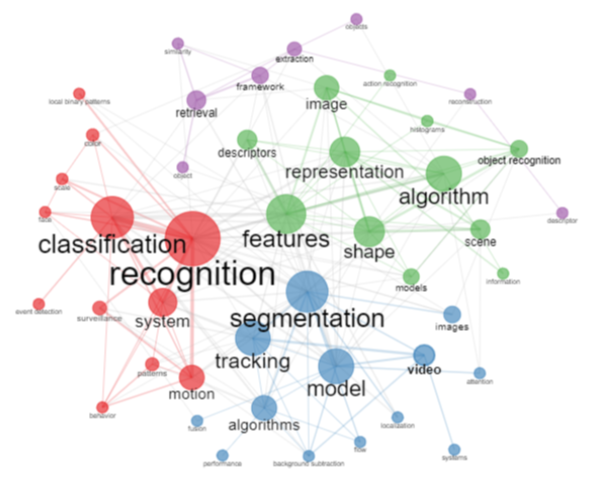
\includegraphics[width=1\textwidth]{experiments/ngsylar/PesqBibliogr/Imagens/ASADES-CoOccurrenceNetwork.png}
    \caption{Rede de Co-ocorrências de maior peso no dataset ASADES@ngsylar.}
    \label{fig:evol:anual:cotonet:ASADES@ngsylar}
\end{figure}

\section{Análise dos dados}

Foi aplicado um filtro ao dataset inicial com 775 registros e mantidos apenas os registros de artigos publicados em revistas científicas. Após a aplicação do filtro, 702 registros foram mantidos no dataset, que a partir desse ponto será idetificado pelo nome ASADES@ngsylar (Articles about Scene Analysis and Description).

\subsection{Análise descritiva do dataset ASADES@ngsylar}

As informações gerais sobre o dataset ASADES@ngsylar de 702 registros são as seguintes:

\begin{description}
\item [\textit{Timespan}] Os artigos no dataset ASADES@ngsylar que atenderam aos critérios de busca e filtragem foram publicados a partir de 1984 e até 2022.

\item [\textit{Sources (Journals, Books, etc)}] Foram 262 fontes de informação que publicaram os documentos recuperados no dataset ASADES@ngsylar. Em média, cada fonte publicou 2,1 artigos. Contudo, o valor da média pode não refletir bem a quantidade real de cada informação geral apresentada.

\item [\textit{Average years from publication}] A média do tempo de publicação dos artigos no dataset ASADES@ngsylar é de 8,64 anos.

\item [\textit{Average citations per documents}] Cada artigo no dataset ASADES@ngsylar foi citado, em média 32,23 vezes.

\item [\textit{Average citations per year per doc}] Cada artigo no dataset ASADES@ngsylar foi citado, em média, 2,9 vezes por ano, após a publicação.

\item [\textit{References}] A quantidade total de referências citadas contidas no dataset ASADES@ngsylar é 25277.

\item [\textit{Keywords Plus (ID)}] 1156 palavras-chave distintas foram encontradas no dataset ASADES@ngsylar.

\item [\textit{Author’s Keywords (DE)}] 2733 palavras-chave distintas foram indicadas pelos autores com artigos presentes no dataset ASADES@ngsylar.

\item [\textit{Authors}] No total, 2381 distintos nomes de autores foram encontrados no dataset.

\item [\textit{Author Appearances}] Os 2381 distintos nomes aparecem 2629 vezes como autores de artigos.

\item [\textit{Authors of single-authored documents}] 34 dos 2381 distintos nomes de autores editaram pelo menos um artigo individualmente.

\item [\textit{Authors of multi-authored documents}] 2347 dos 2381 distintos nomes de autores editaram artigos em colaboração com outros autores.

\item [\textit{Single-authored documents}] Dos 702 artigos no dataset ASADES@ngsylar, 34 foram escritos por um único autor.

\item [\textit{Documents per Author}] Em média, cada autor publicou 0,29 artigos.

\item [\textit{Authors per Document}] Em média, cada documento presentes no dataset ASADES@ngsylar foi escrito por 3,39 autores.

\item [\textit{Co-Authors per Documents}] Em média, as aparições de nomes de autores são distribuídos por 3,75 vezes para os 702 documentos do dataset ASADES@ngsylar.

\item [\textit{Collaboration Index}] Em média, os nomes de autores editaram cerca de 3,5 artigos em colaboração a um ou mais autores.
\end{description}

\subsection{Evolução da Produção Científica}

Com um crescimento anual de 9.05\%, a curva mostra uma tendência de crescimento, embora a variação da quantidade de artigos publicados por ano até o momento seja considerável e a quantidade de artigos publicados não seja suficiente para aproximar a curva a uma curva exponencial.

\begin{figure}[H]
    \centering
    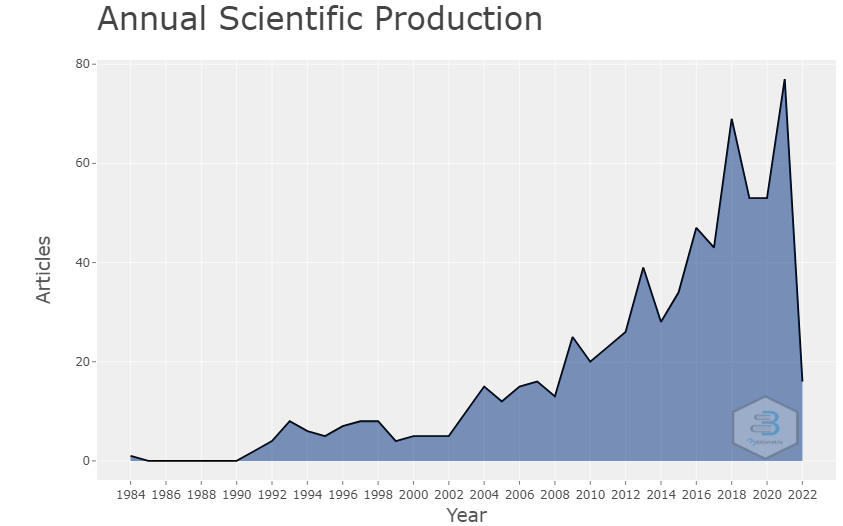
\includegraphics[width=1\textwidth]{experiments/ngsylar/PesqBibliogr/Imagens/ASADES-AnnualScientificProduction.png}
    \caption{Evolução da produção científica no dataset ASADES@ngsylar.}
    \label{fig:evol:anual:ASADES@ngsylar}
\end{figure}

\subsubsection{Interpretação do Crescimento} 

Como visto na figura \ref{fig:evol:anual:ASADES@ngsylar}, a taxa de crescimento do dataset ASADES@ngsylar sugerem que o tema de pesquisa na área de análise e descrição de vídeos tem despertou interesse de forma modesta nos primeiros anos, seguido de um crescimento mais acentuado nos anos seguintes e com tendência de crescimento nos próximos anos. O tema, porém, não parece estar entre as áreas de maior interesse no contexto de produção científica.

\subsection{Evolução das Citações}

A partir do gráfico na figura \ref{fig:evol:anual:citacoes:ASADES@ngsylar}, é visto que não existe muita estabilidade na curva do número de citações, que variava por cerca de 0 a 4 citações por ano e passou a variar de 2 a 6 citações a partir do ano 2000. O pico de quase 30 citações no ano de 1984 provavelmente deve-se a presença de um artigo no dataset publicado neste período e que foi bastante citado.

\begin{figure}[H]
    \centering
    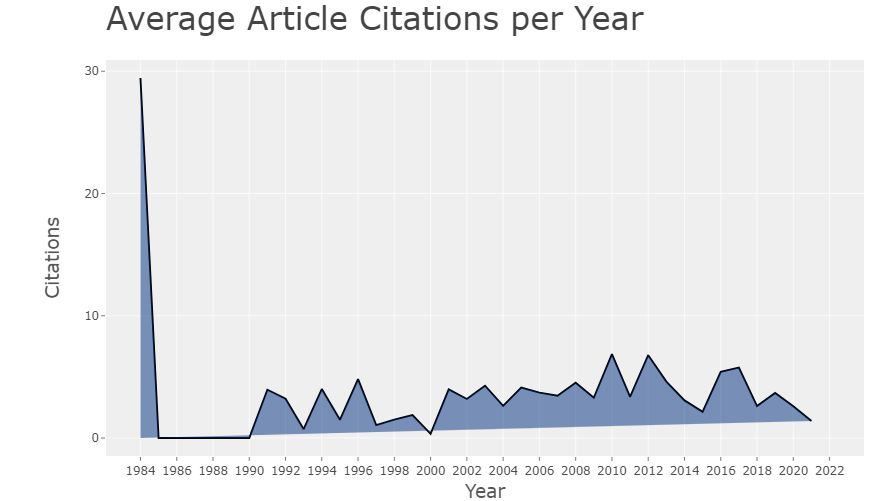
\includegraphics[width=1\textwidth]{experiments/ngsylar/PesqBibliogr/Imagens/ASADES-CitationsYear.png}
    \caption{Evolução das citações no dataset ASADES@ngsylar.}
    \label{fig:evol:anual:citacoes:ASADES@ngsylar}
\end{figure}

\subsubsection{Interpretação das Citações}
Dado o crescimento de produção científica na área, o modesto crescimento na média de citações a cada 20 anos sugere uma tendência de crescimento da bibliografia. Entretanto, deve-se observar com cautela o comportamento da curva nos próximos anos, visto que houveram momentos de queda bruscas na última década.


\subsection{\textit{Plotagem de Três Campos (Diagrama de Sankey)}}
A figura \ref{fig:ASADES@ngsylar:ThreeFieldPlot} apresenta a afinidade entre três diferentes conjuntos de atributos que se correlacionam entre si, sendo estes as 20 citações mais frequentes, os 20 mais proeminentes e as palavras-chaves mais frequentes, da esquerda à direita respectivamente.

\begin{figure}[H]
    \centering
    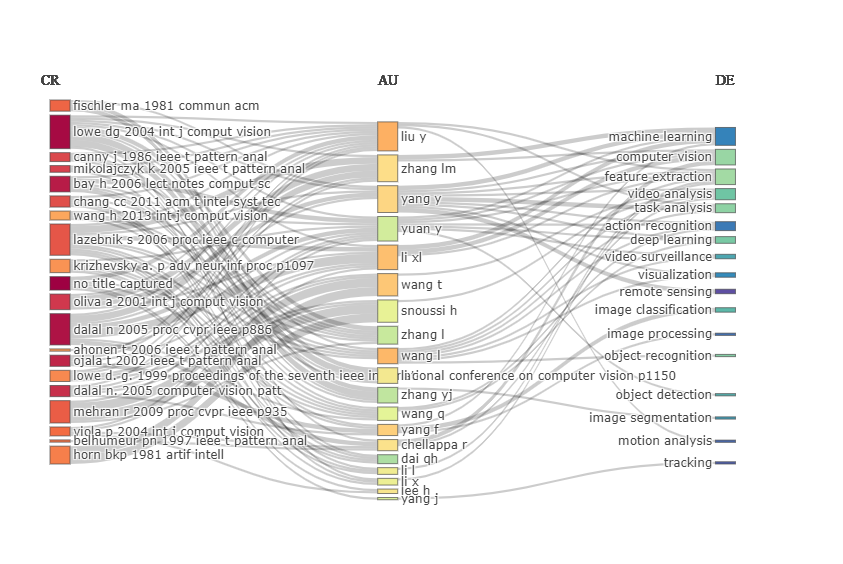
\includegraphics[angle=0,width=1\textwidth]{experiments/ngsylar/PesqBibliogr/Imagens/ASADES-TFPRefAutKeyw.png}
    \caption{Plotagem ``Três Campos'' do dataset ASADES@ngsylar: 20 Autores para Referências e Palavras-Chave mais proeminentes.}
    \label{fig:ASADES@ngsylar:ThreeFieldPlot}
\end{figure}

\subsubsection{Interpretação do diagrama da figura \ref{fig:ASADES@ngsylar:ThreeFieldPlot}}
Os termos mais recorrentes são \textit{machine learning} e \textit{computer vision}, seguidos por termos como \textit{video analysis}, o que sugere a relevância da aplicação de inteligência artificial e apredizado de máquina no processo de análise de vídeo e classificação de imagens.
Aguns outros termos como \textit{object recognition} aparecem em menor escala, indicando a aplicação de estudos baseados no tema para analise de imagens capturadas em tempo real por robôs.
O lado esquerdo do diagram sugere alguns dos artigos mais relevantes para embasamento de estudos relacionados ao tema de análise e descrição de vídeos.

\subsection{Análise Bibliométrica}

\subsubsection{Fontes de Informação}

\begin{figure}[H]
    \centering
    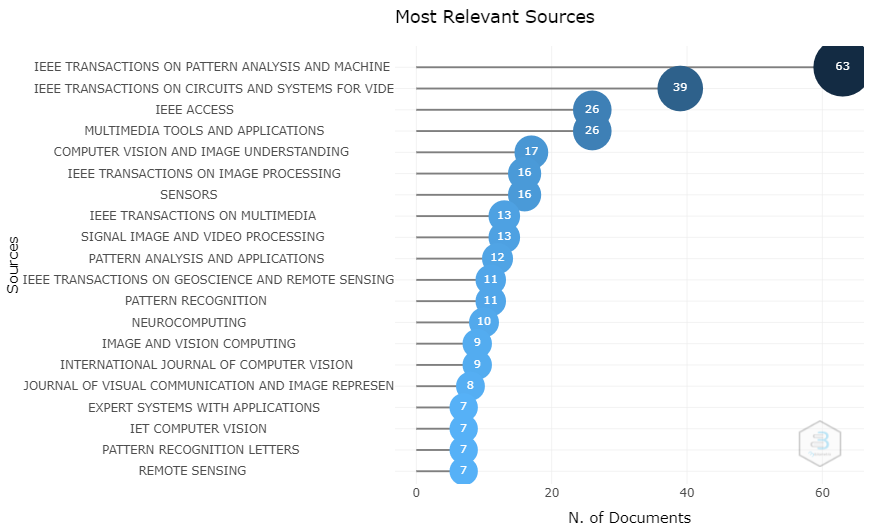
\includegraphics[angle=0,width=1\textwidth]{experiments/ngsylar/PesqBibliogr/Imagens/ASADES-MostRelevantSources.png}
    \caption{Fontes de Informação mais Relevantes no dataset ASADES@ngsylar.}
    \label{fig:ASADES@ngsylar:RelevantSources}
\end{figure}

A figura \ref{fig:ASADES@ngsylar:RelevantSources} mostra as principais fontes de informação onde se encontram os artigos presentes no dataset ASADE@ngylar, destacando as \textit{IEEE Transactions on Pattern Analysis and Machine} e \textit{IEEE Transactions on Circuits and Systems for Vide}.

\subsubsection{Autores}

\begin{figure}[H]
    \centering
    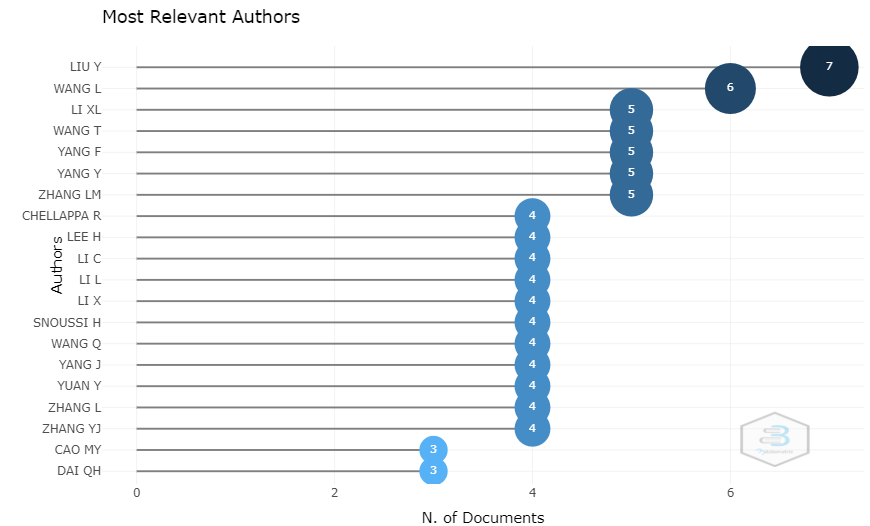
\includegraphics[angle=0,width=1\textwidth]{experiments/ngsylar/PesqBibliogr/Imagens/ASADES-MostRelevantAuthors.png}
    \caption{Nomes de autores com maior relevância no dataset ASADES@ngsylar.}
    \label{fig:ASADES@ngsylar:RelevantAuthors}
\end{figure}

A figura \ref{fig:ASADES@ngsylar:RelevantAuthors} sugere quais são os autores mais relevantes e com maior número de artigos publicados presentes no dataset ASADE@ngylar. Faz-se necessário entretanto analisar mais profundamente a relação que cada um dos autores tem com tema.

\subsubsection{Países citados}

\begin{figure}[H]
    \centering
    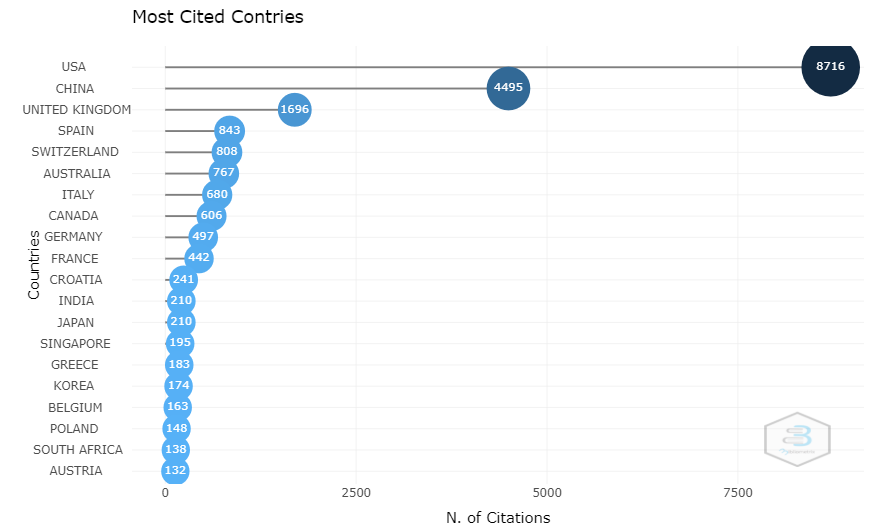
\includegraphics[angle=0,width=1\textwidth]{experiments/ngsylar/PesqBibliogr/Imagens/ASADES-MostCitedCountries.png}
    \caption{Países mais citados no dataset ASADES@ngsylar.}
    \label{fig:ASADES@ngsylar:MostCitedCountries}
\end{figure}

Na figura \ref{fig:ASADES@ngsylar:MostCitedCountries}, entre os países mais citados, é visto que maior parte da produção encontra-se nos Estados Unidos, seguido pela China e logo após pelo Reino Unido.

\subsubsection{Estrutura Intelectual}

\begin{figure}[H]
    \centering
    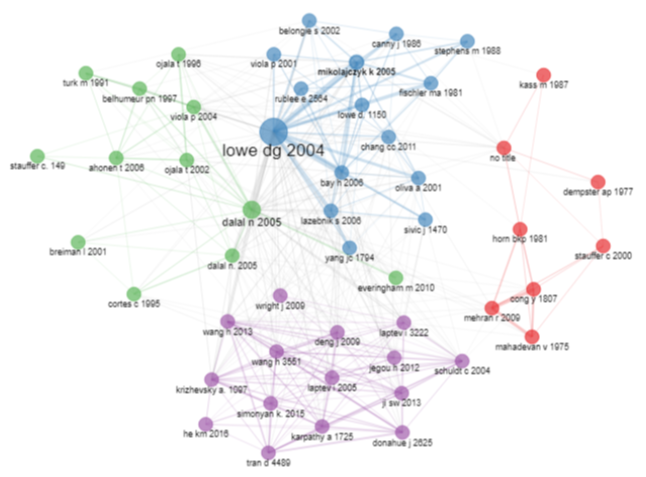
\includegraphics[angle=0,width=1\textwidth]{experiments/ngsylar/PesqBibliogr/Imagens/ASADES-Intelect.png}
    \caption{Países mais citados no dataset ASADES@ngsylar.}
    \label{fig:ASADES@ngsylar:StIntel}
\end{figure}

A figura \ref{fig:ASADES@ngsylar:StIntel} mostra a rede de co-citação de artigos no conjunto de dados ASADES@ngsylar. São observados quatro aglomerados principais, dentre os quais o aglomerado azul se destaca como mais importante, com o trablho de Lowe dg, no qual grande parte dos artigos se baseia com peso e buscam encontrar métodos eficientes de extração de características ou padrões que não variam e podem ser identificadas em diferentes pontos de vista de um objeto ou cena capturada num dado ambiente.

\section{Conclusão}
Dadas as questões iniciais, percebemos que grande parte dos artigos encontrados não tem o foco principal sobre a descrição de vídeos, embora a maior parte tenho bases no tocande à análise de vídeo e reconhecimento de padrões em vídeo e processamento e identificação de imagens. Fica constatado que o tema pesquisado ainda não é um tema de forte engajamento ou com uma gama muito alta de autores interessados, mas é possível observar um modesto crescimento no número de publicações na área ou em contextos similares.

Dentre as técnicas observadas no estudo bibliométrico e leitura dos resumos de alguns dos artigos considerados mais relevantes, fica claro a maior parte dos estudos e experimentos feitos na área de análise e descrição de vídeo estão fortemente apoiadas em \textit{machine learning}, ou aprendizado de máquina. É possível ver que existe também certas bases em algoritmos de processamento de imagens e reconhecimento de ação ou movimentação em vídeo para descrever ou classificar o conteúdo em uma tela de vídeo ou câmera.

Os países mais engajados na produção de artigos científicos no abordado tema são os Estados Unidos e em seguida a China. Alguns outros países também apresentam uma considerável relevância na área de pesquisa e produção científica, como é o caso do Reino Unido e da Espanha.

Por fim, vê-se uma certa dispersão em certos artigos a respeito da abordagem do tema, como é o caso de alguns que tem objetivo maior em aplicação de análise de vídeo para locomoção ou aplicação em si a robôs físicos. A quantidade de artigos ainda é pequena, e a área pouco explorada, existe espaço suficiente para áreas como a robótica explorar técnicas e funcionalidades mais voltadas a direção do tema.



\bibliographystyle{plainnat}
\bibliography{RESIC}

\end{document}.
